\documentclass[11pt]{article}
\usepackage[a4paper,margin=1in]{geometry}
\usepackage{fontspec}
\usepackage{xeCJK}
\usepackage{graphicx}
\usepackage{caption}
\usepackage{booktabs}
\usepackage{microtype}
\usepackage{parskip}

\setmainfont{Times New Roman}
\setsansfont{Arial}
\setCJKmainfont{Songti SC}
\setCJKsansfont{STHeiti}

\title{传统事件表示 Baseline 数据分析}
\author{}
\date{}

\begin{document}
\sloppy
\maketitle

\paragraph{核心结论：传统方法不是弱下界。} 从已经完成的 N-MNIST、N-Caltech101 和 MVSEC 三条实验线看，传统事件表示并没有表现为简单的低性能参照组，而是在统一下游模型和统一评估协议下保持了可比较的竞争力。分类任务中，N-MNIST 已经接近饱和，五种传统方法中有四种超过 98.0\% 测试准确率；其中 Voxel Grid 达到最高的 99.08\%，测试损失也最低，为 0.034060。N-Caltech101 更能区分表示能力，Timestamp Image 达到最高测试准确率 52.9277\%，并且是该数据集上耗时最短的方法，运行时间为 793.65 秒。MVSEC optical flow 中，在 11 个方法完全共享训练集、测试集、窗口大小、stride、EVFlowNet-like decoder 和 early stopping 设置的前提下，Timestamp Image 得到最低 AEE 2.791623 和最低 outlier rate 36.608703\%。因此，目前数据支持的谨慎结论是：传统表示在已有分类和光流协议下是强 baseline，而不是可以被忽略的简单下界。

\begin{figure}[t]
  \centering
  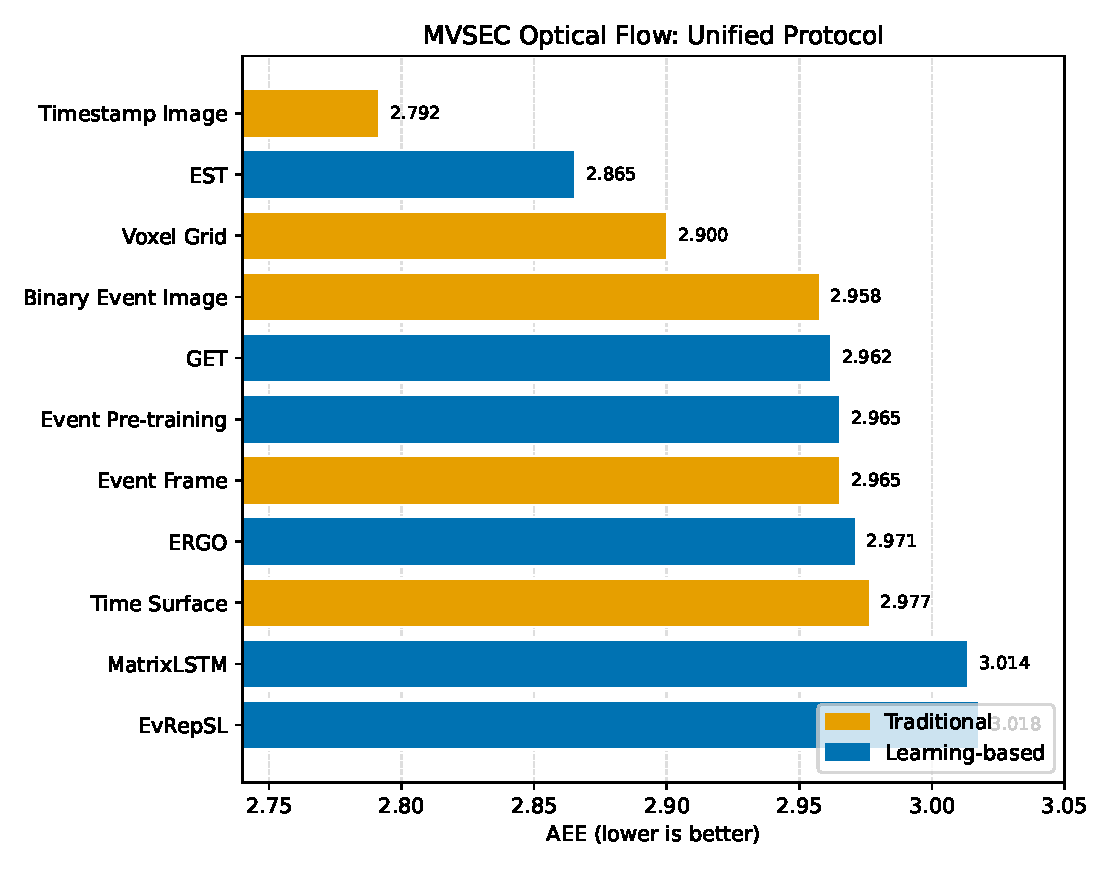
\includegraphics[width=0.92\linewidth]{mvsec_aee_horizontal_bar.pdf}
  \caption{MVSEC optical flow 统一协议下的 AEE 对比。横向条形图按 AEE 排序，AEE 越低越好。橙色表示 traditional 方法，蓝色表示 learning-based 方法。由于所有方法的 AEE 集中在 2.79 到 3.02 之间，横轴采用局部放大尺度以呈现细微差异。}
  \label{fig:mvsec-aee-bar}
\end{figure}

\paragraph{核心结论：MVSEC 上 Timestamp Image 形成最强单次结果。} 图 \ref{fig:mvsec-aee-bar} 显示，在 MVSEC 原始协议式划分中，Timestamp Image 的 AEE 为 2.791623，低于最佳 learning-based 方法 EST 的 2.865447，差值为 0.073824，相对于 EST 约为 2.576\% 的 AEE 下降。同时，Timestamp Image 的 outlier rate 为 36.608703\%，也低于 EST 的 37.039154\%。这个结果需要严格限定在当前统一 benchmark 协议内解释，因为这些 learning-based 方法没有使用各自论文原始的完整训练栈，而是接入同一个 EVFlowNet-like decoder。即便如此，该结果仍然说明：在光流估计任务中，保留最新事件时间信息的简单传统表示可以提供非常有效的运动线索，并不必然弱于更复杂的学习型表示。

\paragraph{核心结论：通道数和表示复杂度没有单调收益。} MVSEC 结果并不支持“表示越复杂、通道越多，性能越好”的简单判断。Timestamp Image 仅使用 2 个输入通道，却取得最低 AEE；EST 使用 18 个通道，排名第二；Voxel Grid 使用 10 个通道，AEE 为 2.900117，排名第三；GET 使用 24 个通道，但 AEE 为 2.961931。更具体地，Event Frame 和 Event Pre-training 都是 2 通道表示，两者 AEE 分别为 2.965373 和 2.965345，几乎没有可解释的差异。这个现象提示，当前协议下决定性能的关键可能不是通道数量本身，而是时间信息如何被保留、压缩并送入下游 decoder。

\begin{figure}[t]
  \centering
  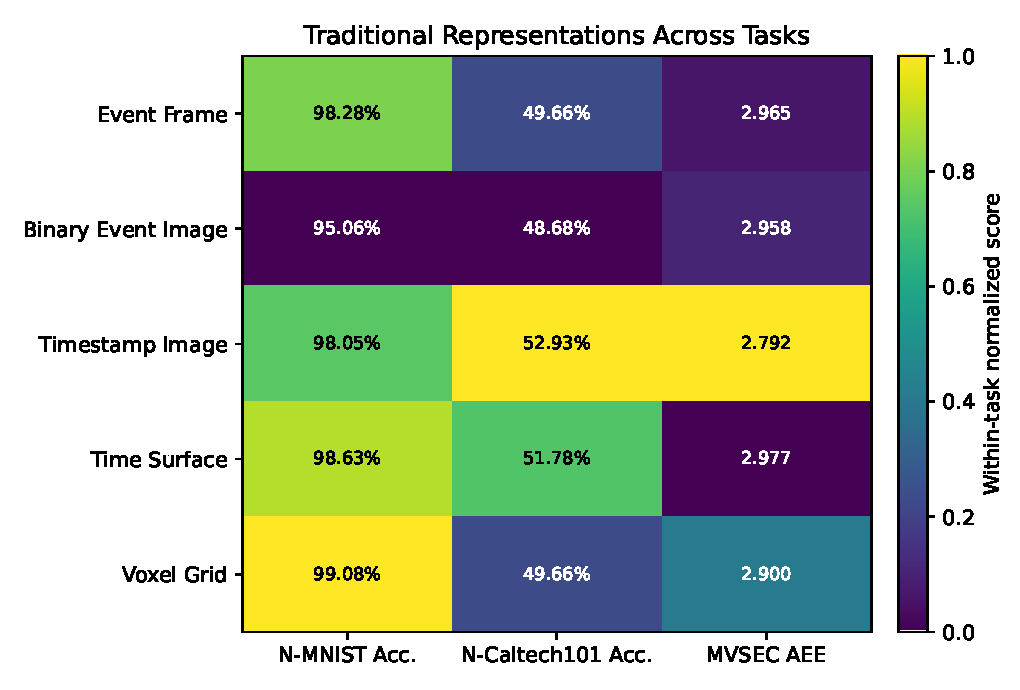
\includegraphics[width=0.82\linewidth]{traditional_cross_task_heatmap.pdf}
  \caption{传统表示在三个任务上的任务内归一化表现。颜色表示同一任务内部的相对分数，颜色越深代表该任务内表现越好；格子中的文本保留原始指标。N-MNIST 和 N-Caltech101 使用 accuracy，越高越好；MVSEC 使用 AEE，越低越好，因此热力图颜色对 MVSEC 做了反向归一化。}
  \label{fig:cross-task-heatmap}
\end{figure}

\paragraph{核心结论：最佳传统表示具有明显任务依赖性。} 图 \ref{fig:cross-task-heatmap} 展示了一个跨任务趋势：传统方法中不存在一个在所有任务上稳定占优的单一表示。Voxel Grid 在 N-MNIST 上最好，准确率为 99.08\%；但在 N-Caltech101 上，Timestamp Image 以 52.9277\% 排名第一，Time Surface 以 51.7796\% 排名第二，而 Voxel Grid 的测试准确率为 49.6556\%。在 MVSEC 上，Timestamp Image 继续取得最优 AEE 2.791623，Voxel Grid 则为 2.900117。这个变化说明，N-MNIST 的短时数字识别更受益于极性分离的时间分箱累积，而 N-Caltech101 和 MVSEC 更依赖 timestamp 或 recency 相关的信息保留。换言之，传统表示的选择应当由任务的时空结构决定，而不是简单固定使用某一个 baseline。

\paragraph{核心结论：效率和精度之间存在非平凡权衡。} 从分类结果看，Timestamp Image 的效率优势比较突出。N-MNIST 上，Timestamp Image 是最快方法，耗时 786.48 秒，测试准确率为 98.05\%；Voxel Grid 的准确率更高，为 99.08\%，但耗时 1266.66 秒。Event Frame 耗时 2365.40 秒，却只达到 98.28\%，说明更长训练时间并没有带来相应收益。N-Caltech101 上，Timestamp Image 同时取得最高准确率 52.9277\% 和最低运行时间 793.65 秒，是该任务中最清晰的效率--性能优势点。MVSEC 上，Timestamp Image 和 EST 都在第 1 个 epoch 达到最佳验证 checkpoint，并在 11 个 epoch 后 early stop；Voxel Grid 则在第 13 个 epoch 达到最佳验证 AEE，并在 23 个 epoch 后停止。由此可见，报告中不应只展示最终指标，还应保留训练曲线和 early stopping 信息，以体现方法的收敛效率。

\paragraph{核心结论：报告表述应避免过度声称。} 当前结果可以支持“传统 baseline 在统一协议下具有竞争力”这一结论，但不能支持“传统方法全面优于 learning-based 方法”或“达到 SOTA”这类泛化表述。原因有三点：第一，N-MNIST 和 N-Caltech101 目前只有 traditional baseline，没有对应 learning-based 分类结果进入同一表格；第二，MVSEC 虽然完成了 traditional 和 learning-based 的统一比较，但使用的是共享 decoder，而不是各篇论文原始训练系统；第三，GEN1 detection 尚未完成，因此不能对检测任务做数据驱动结论。最严谨的写法是：在已完成的分类和光流实验中，timestamp-preserving traditional representations 显示出稳定竞争力；未来需要补齐 GEN1 和对应 learning-based 分类结果，才能形成四任务完整 benchmark 结论。

\end{document}
